\subsection{Glyph: \glyph{Modulation}}
\label{sec:modulation}

A general modulation where the exact nature of the modulation is not specified or not known.
The \glyph{modulation} glyph can be used when one does not know the precise sign of the effect (stimulation or inhibition).

\begin{glyphDescription}

\glyphSboTerm
SBO:0000168 ! control

\glyphOrigin
One \glyph{EPN} (\sect{EPNs}) or  \glyph{logical operator} (\sect{logic}).

\glyphTarget
One \glyph{process node} (\sect{PNs}).

\glyphSymbol
The target extremity of a \glyph{modulation} carries an empty diamond, as shown in \fig{modulation}.

\end{glyphDescription}

\begin{figure}[H]
  \centering
  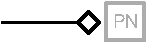
\includegraphics{images/build/modulation.pdf}
  \caption{The \PD glyph for \glyph{modulation}.}
  \label{fig:modulation}
\end{figure}

\fig{modul-nico} represents the effect of nicotine on the process between closed and open states of a nicotinic acetylcholine receptor. High concentrations of nicotine open the receptor while low concentrations can desensitize it without opening.

\begin{figure}[H]
  \centering
  \includegraphics[scale = 0.8]{images/build/modulation_nAChR_example.pdf}
  \caption{Modulation of nicotinic receptor opening by nicotine.}
  \label{fig:modul-nico}
\end{figure}
